\section{Messwerte und Auswertung}

\subsection{Sinusgitter} %fertig

Der Laser wird anhand des 2. Spiegels zentriert, dann werden das Sinusgitter und der Schirm eingebaut. Die Distanz zwischen den beiden Maxima 1. Ordnung ergibt sich aus der $x$- und der $y$-Verschiebung auf dem Schirm. Wir haben folgende Werte gemessen:
\begin{itemize}
\item $D_x = (9.9 \pm 0,1) cm$ (Distanz in $x$-Richtung)
\item $D_y = (1.1 \pm 0.1) cm$ (Distanz in $y$-Richtung)
\item $L = (5.9 \pm 0.3) cm$ (Distanz zwischen dem Gitter und dem Schirm)
\end{itemize}

Aus $D_x$ und $D_y$ ergibt sich die Distanz $D=\sqrt{D_x^2 + D_y^2} = 9.96$ mit dem Fehler
$$\sigma_D = \sqrt{\left(\frac{\partial D}{\partial D_x}\right)^2\sigma_{D_x}^2 + \left(\frac{\partial D}{\partial D_y}\right)^2\sigma_{D_y}^2} = \sqrt 2 \left(\frac{\partial D}{\partial D_x}\right)\sigma_{D_x} = \sqrt 2 \frac{D_x}{\sqrt{D_x^2 + D_y^2}}\sigma_{D_x} = \sqrt 2 \frac{D_x}{D}\sigma_{D_x} = 0,14$$

Somit: $$\boxed{D = (9.96 \pm 0.14) cm}$$

Es folgt der Winkel $\alpha$ aus $\tan(\alpha) = \frac{D}{2L} \Leftrightarrow\alpha = \arctan\left(\frac{D}{2L}\right) = 40.17^\circ$ mit dem Fehler

$$\sigma(\alpha) = \sqrt{\left(\frac{\partial \alpha}{\partial D}\right)^2\sigma_{D}^2 + \left(\frac{\partial \alpha}{\partial L}\right)^2\sigma_{L}^2} = \sqrt{\frac{L\sigma_D^2 + D\sigma_L^2}{2L(1+D^2/4L^2)}} = 0.22^\circ$$

Es folgt: $$\boxed{\alpha = (40.17 \pm 0.22)^\circ = (0.701 \pm 0.004) rad} $$

Die Gitterkonstante $K$ l\"asst sich somit berechnen: $$ K\sin(\alpha) = n\lambda \Leftrightarrow K = \frac{n\lambda}{\sin(\alpha)} = 9810.13 \ \mathring A \ \text{mit \ } n=1$$

$K$ besitzt den Fehler (unter Vernachl\"assigung des Fehlers auf $\lambda$): $$\sigma_K = \sqrt{\left(\frac{\partial K}{\partial \alpha}\right)^2\sigma_\alpha^2} = \frac{\lambda\cos(\alpha)\sigma_\alpha}{\sin^2(\alpha)} = 44.62 \ \mathring A$$

Somit folgt: $$\boxed{K=(9810 \pm 44) \ \mathring A = (981.0 \pm 4.4) \ nm}$$

Als Vergleich: Auf dem Gitter ist die Zahl der Linien pro Millimeter angegeben: \\ $g_{theo}=1016 L/mm$. Es folgt der Wert f\"ur die Gitterkonstante: $K_{theo} = 1/g_{theo} = 9842.52 \ \mathring A$, welcher sehr dicht an unserem ermittelten Wert liegt und innerhalb der ersten Standardabweichung.

\subsection{Bestimmung der Gitterkonstanten}

Wir haben den Strahlengang wie in 3.2.2 beschrieben justiert um eine m\"oglichst hohe Genauigkeit bei unserer Messung zu erhalten.

\subsubsection{Eichung anhand des Gitters R}

Sei $\Delta t$ die zeitliche Distanz zwischen 2 Nebenmaxima der Intensit\"atsverteilung. Die Distanz zwischen dem Hauptmaximum und einem Nebenmaximum ist somit $\Delta t/2$ und ist proportional zu $\sin(\alpha)$. Es gilt: $$\sin(\alpha) = \frac{n\lambda}{K} = \gamma \frac{\Delta t}{2}$$
Wir bestimmen die Proportionalit\"atskonstante $\gamma$ durch lineare Regression, indem wir $\Delta t/2$ gegen $n$ auftragen und den Steigungsfaktor $b$ ermitteln. Der Achsenabschnitt $a$ sollte idealerweise Null sein.

\begin{center}
\begin{tabular}{lllll}
\toprule
Peak & t in $\mu s$ & st in $\mu s$ & $\Delta t$ in $\mu s$ & $s\Delta t$ in $\mu s$ \\
\midrule
0. Ordnung \\
 & 501,0635 & 3,36E-002\\
\midrule
1. Ordnung\\
links & 404,7489 & 3,71E-002 & 192,4441 & 7,29084668847E-002\\
rechts & 597,193 & 3,59E-002\\
\midrule
2. Ordnung\\ 
links & 309,3735 & 2,07E-001 & 383,268 & 3,90324905236E-001\\
rechts & 692,6415 & 1,83E-001\\
\midrule
3. Ordnung\\ 
links & 214,3283 & 5,28E-001 & 573,2411 & 1,21769040489\\
rechts & 787,5694 & 6,89E-001\\
\bottomrule
\end{tabular}
\end{center}

Die Parameter der linearen Regression:
$$ b               = (9.53491e-05      \pm 9.823e-08) s    (0.103\%) $$
$$ a               = (8.74055e-07      \pm 1.043e-07) s    (11.94\%) $$

Der Achsenabschnitt $a$ ist also tatsächlich um einige zwei Größenordnungen kleiner als die Steigung $b$ und wird daher vernachlässigt. Somit erhalten wir den Zusammenhang

$$\frac{\Delta t}{2} = \frac{\lambda}{K\gamma}n = b\cdot n$$

den wir umstellen können nach $\gamma$, dem Proportionalitätsfaktor zwischen Zeit $t$ und Sinus des Winkels $\sin \alpha$ 

$$ \gamma = \frac{\lambda}{Kb} = (53.093317084272421 \pm 0.0546974909799) s^{-1} $$
%$$s\gamma = \frac{\lambda}{Kb^2} \cdot sb $$


\subsubsection{Bestimmung der Gitterkonstanten f\"ur die 5 Gitter}

Mit diesem Faktor können wir nun die Gitterkonstanten der anderen fünf Gitter aus dem Abstand der Maxima der ersten Ordnung bestimmen:
$$ g = \frac{\beta}{\lambda}\cdot \frac{\Delta t}{2} \text{ bzw. } k = \frac{2 \lambda }{\beta \Delta t} $$
\begin{center}
\begin{tabular}{lllll}
\toprule 
Gitter & $\Delta t /2$ in $\mu s$ & $s\Delta t /2$ in $\mu s$ & $k$ in $\mu m$ & $sk$ in $\mu m$\\
\midrule
G1 & 89.742 & 0.568 & 132.81 & 0.85\\
G3 & 112.111 & 0.205 & 106.31 & 0.22\\
G4 & 112.411 & 0.107 & 106.03 & 0.14\\
08540 & 113.490 & 0.677 & 105.02 & 0.64\\
08534 & 91.0123 & 0.139 & 130.96 & 0.24\\
\bottomrule
\end{tabular} 
\end{center}

F\"ur die beiden PHYWE-Gitter kennen wir den theoretischen Wert, n\"amlich: 
\begin{itemize}
\item PHYWE-08534: $g_{theo} = 8 L/mm\ \Rightarrow \ K_{theo} = 125 \ \mu m$
\item PHYWE-08540: $g_{theo} = 10 L/mm\ \Rightarrow \ K_{theo} = 100 \ \mu m$
%Vergleich mit dem exp. ermittelten Wert
\end{itemize} 

\subsection{Berechnung der Aperturfunktion f\"ur Gitter 1}

Wir nähern die Aperturfunktion mittels den Intensit\"aten der gemessenen Verteilung als Fourierreihe:
$$g(x) = \frac{\sqrt{I_0}}{2} + \sum_{n=1}^N \sqrt{I_n}\cos\left(\frac{2\pi n}{K}x \right)$$
F\"ur die $I_n$ haben wir folgende Werte ermittelt:

%Resultate I_0
\begin{tabular}{lll}
 \toprule
Ordnung & Amplitude & Fehler \\
\midrule
0. Ordnung & 5.5184706157133 & 0.0205159936960068 \\
1. Ordnung l & 0.221293372204415 & 0.00303468123804445 \\
1. Ordnung r & 0.154596997473865 & 0.00250997613519101 \\
2. Ordnung l & 0.147836581064078 & 0.00309767922452523 \\
2. Ordnung r & 0.135446035218821 & 0.00287225704831411 \\
3. Ordnung l & 0.0869833409521151 & 0.00328617199395248 \\
3. Ordnung r & 0.0952050159181131 & 0.00267868139085647 \\
\bottomrule
\end{tabular}



Mit $K = 130.96 \mu m $ erhalten wir folgende  
\begin{figure}[h!]
 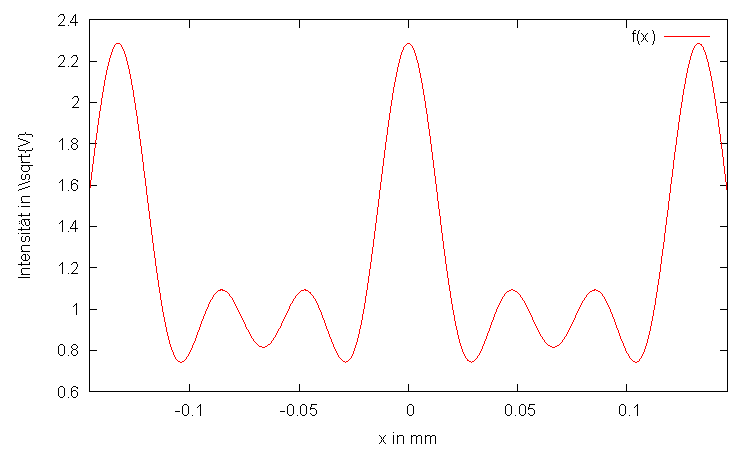
\includegraphics{Bilder/appertur.pdf}
\caption{Apperturfunktion}
\end{figure}


\subsection{Bestimmung des Verh\"altnisses zwischen Spaltbreite und Spaltabstand}

Den maximalen y-Wert erhalten wir für $g\left( 0 \right) = \sqrt{I0}/2+\sqrt{I1}+\sqrt{I2}+\sqrt{I3} = y_{max} = 2.28627 $. Den minimalen y-Wert erhalten wir durch ablesen $ y_{min} = 0.743486 $. Die Halbwertsbreite $b$ mit $ g\left( - b/2 \right) = g \left( b/2 \right) = 1.51488 $ ergibt sich als $ b = 0.027334 $. Somit erhalten wir für das Verhältnis von Spaltbreite zu -höhe
$$ v = \frac{b}{K-b} = 0.26378 $$ %TODO Fehler? 

\subsection{Aufl\"osungsverm\"ogen der Gitter}

Das Aufl\"osungverm\"ogen $a$ ergibt sich bei normalen Gittern durch $a=N\cdot m$, wobei N die Zahl der durchleuchteten Maxima ist, und m die Zahl der sichtbaren Maxima. N bestimmen wir, indem wir die Laserbreite $b_L$ messen und durch die Gitterkonstante $K$ teilen.\\
Die Laserbreite haben wir mit dem Schirm gemessen und haben $b_L = (3.0 \pm 0.5) mm$ erhalten.\\
Es gilt also: $$N = \frac{b_L}{K}$$
mit dem Fehler: $$\sigma_N = \sqrt{\frac{\sigma_{b_L}^2K^2 + \sigma_K^2b_L^2}{K^4}}$$
Der Fehler auf $a$ ist: $$\sigma_a = \frac{\partial a}{\partial N}\sigma_N = m\cdot \sigma_N$$

Somit folgt f\"ur die Gitter:

\begin{itemize}
\item Gitter 1: $ a = 67.76575165317837 \pm 11.302658636724754 $
\item Gitter 3: $ a = 56.437974555788117 \pm 9.4070743547623081 $
\item Gitter 4: $ a = 28.294658556680321 \pm 4.7159427734459909 $
\item PHYWE 08540: $ a = 28.566288540708861 \pm 4.764184123944938 $
\item PHYWE 08534: $ a = 45.816820585847005 \pm 7.6366043023007304 $
\end{itemize}


\subsection{Raman-Nath-Theorie}

Durch Ablesen haben wir die Intensität der Maxima bestimmt. Diese haben wir dann mit der Intensität des Hauptmaxima bei ausgeschalteter Spannung $I_0 = $ normiert. Die in der Anleitung empfohlene Verwendung des 1. Minimums bei der Nullten Ordnung zur Bestimmung des Skalierungsfaktors $ $ konnten wir leider nicht befolgen, da dieses Minimum bei nicht durch unsere Messwerte abgedeckt wurde. Daher haben wir den Faktor alternativ durch Fitten der Funktion $J_0(a_0*x)$ an die 0. Ordnung bzw. $J_1(a_1*x)$ an die 1. Ordnung ermittelt. Wir erhalten dabei $a_0 = 1.8453e-01 \pm 3.7e-04$ sowie $a_1 = 2.3449e-01 \pm 7.0e-04 $ und verwenden für die restlichen beiden Ordnungen den Mittelwert $a = 2.09508e-01$. 

\begin{figure}[ht!]
 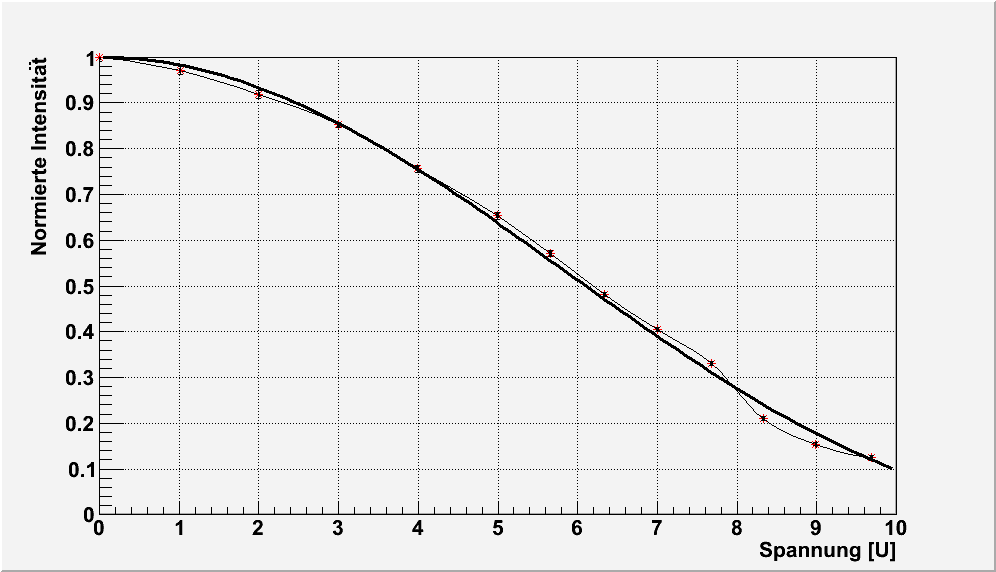
\includegraphics[width=0.9\textwidth]{Bilder/raman/raman-fit_0.png}
 \caption{Vergleich 0. Beugungsordnung mit $J_0^2$}
\end{figure}

\begin{figure}[ht!]
 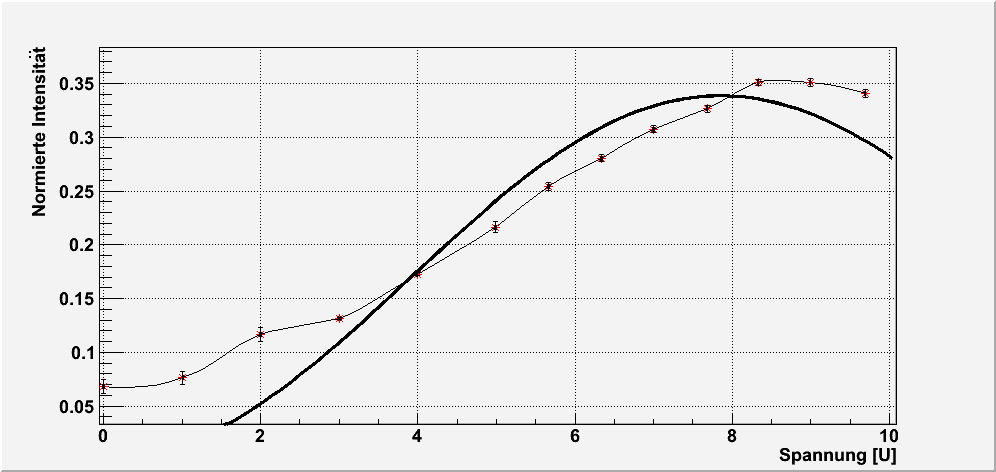
\includegraphics[width=0.9\textwidth]{Bilder/raman/raman-fit_1.png}
 \caption{Vergleich 1. Beugungsordnung mit $J_1^2$}
\end{figure}

\begin{figure}[ht!]
 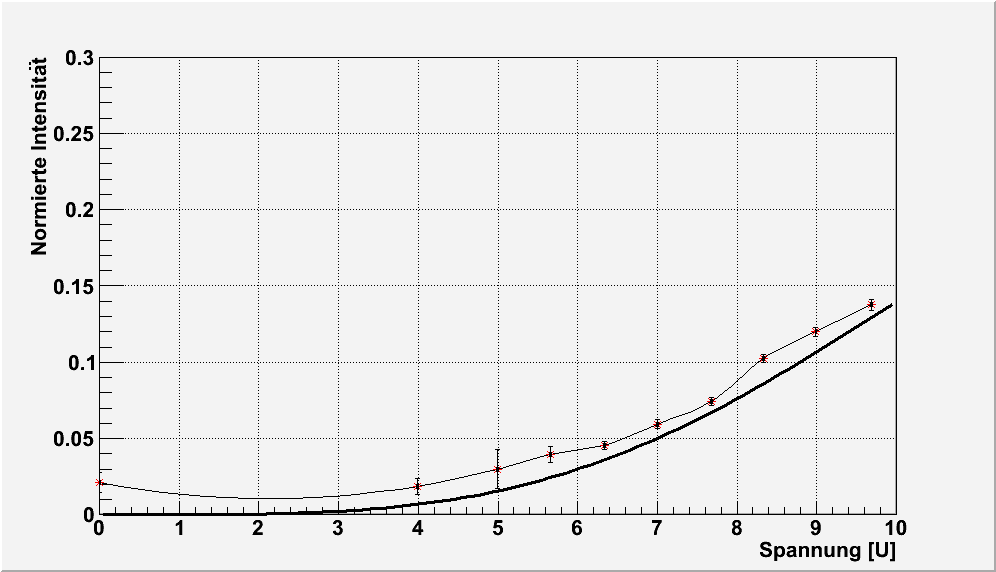
\includegraphics[width=0.9\textwidth]{Bilder/raman/raman-fit_2.png}
 \caption{Vergleich 2. Beugungsordnung mit $J_2^2$}
\end{figure}

\begin{figure}[ht!]
 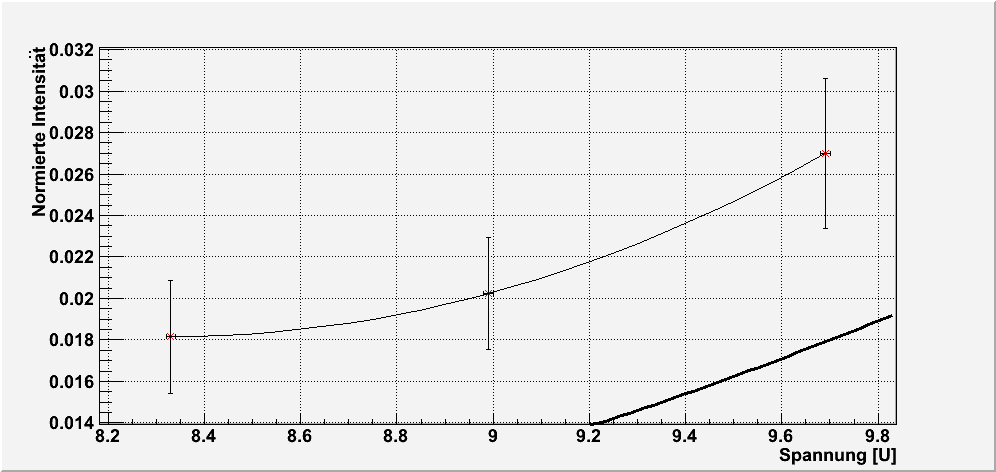
\includegraphics[width=0.9\textwidth]{Bilder/raman/raman-fit_3.png}
 \caption{Vergleich 3. Beugungsordnung mit $J_3^2$}
\end{figure}


\subsubsection{Ultraschallwellenlänge}

Für die Ermittlung der Schallwellenlänge haben wir die Messung bei $ U = 9.69 V$ und $f = 2109.195 kHz $ verwendet. Dazu haben wir die Zeit $t$ der Maxima gegen ihre Ordnung aufgetragen. Aus der Steigung $a$ einer Ausgleichsgeraden erhalten wir über den Zusammenhang 
$$ \sin \alpha = \frac{m \lambda}{\lambda^{*}} = \beta \frac{\Delta t}{2} $$
 die Schallwellenlänge $ \lambda^* $

\begin{center}
\begin{table}[ht!]
\caption{Steigung und Achsenabschnitt der Ausgleichsgeraden}
\begin{tabular}{llll}

\toprule
a & 2.07162e-05   &  $ \pm 9.1e-08$  &    $(0.4392\%)$\\
b & 9.85261e-05 & $ \pm - 1.966e-07$ &   $(0.1995\%)$ \\
\bottomrule
\end{tabular}
\end{table}
\end{center}


Aus $ \beta \frac{\Delta t}{2} = a m + b = \frac{\lambda}{\lambda^*} m + b $ folgt $ \lambda^* = \frac{\lambda}{\beta a} = 575.329 \mu m$ 



$sin \alpha = $













